\begin{problem} {Search and Heuristics}

% $\begin{center} \includegraphics[scale=.33]{figures/movingagent.png} 
% $\end{center}
\begin{center}
    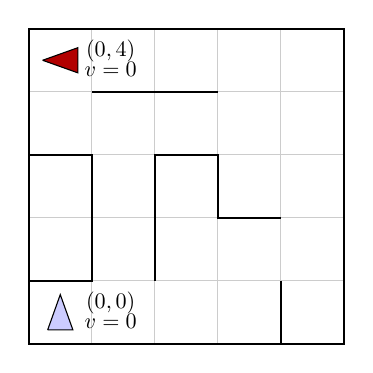
\begin{tikzpicture}[scale=0.8]
    \draw[step=1,gray!40!white,thin] (0,0) grid (5,5);
    \draw[black, thick] (0,0) rectangle (5,5);
    
    \draw[fill=blue!20!white] (0.3, 0.22) -- (0.7, 0.22) -- (0.5, 0.78) -- (0.3, 0.22);
    \draw[fill=red!70!black] (0.22, 4.5) -- (0.78, 4.3) -- (0.78, 4.7) -- (0.22, 4.5);
    \draw[black, thick] (1, 4) -- (3, 4);
    \draw[black, thick] (0, 1) -- (1, 1) -- (1, 3) -- (0, 3);
    \draw[black, thick] (2, 1) -- (2, 3) -- (3, 3) -- (3, 2) -- (4, 2);
    \draw[black, thick] (4, 0) -- (4, 1);

    \node[scale=0.8] at (1.3, 0.65) {$(0, 0)$};
    \node[scale=0.8] at (1.3, 0.35) {$v = 0$};
    \node[scale=0.8] at (1.3, 4.65) {$(0, 4)$};
    \node[scale=0.8] at (1.3, 4.35) {$v = 0$};
    \end{tikzpicture}
\end{center}

Consider a car-like agent trying to navigate out of a maze, similar to the one depicted above. The agent is directional and always faces a specific direction \(d \in (N, S, E, W)\). With each action, the agent has the option to either move forward at a variable speed \(v\) or to turn.

The movement actions include \textit{faster}, \textit{maintain}, and \textit{slower}. When the agent performs these actions, it moves a number of squares corresponding to its \textbf{new} adjusted velocity. Let \(v\) represent the agent's current velocity, and \(v'\) denote the new adjusted velocity.

\begin{itemize}[noitemsep,topsep=0pt]\vspace{-0.3cm}
    \item \textit{Faster}: $v'$ = $v$ + 1
    \item \textit{Slower}: $v'$ = $v$ - 1
    \item \textit{Maintain}: $v'$ = $v$
\end{itemize}

The turning actions are \textit{left} and \textit{right}, which change the agent’s direction by 90 degrees. \textbf{Turning is only permitted when the velocity is zero.} Turning leaves the speed at zero. 
\begin{itemize}[noitemsep,topsep=0pt]\vspace{-0.3cm}
    \item \textit{Left}: change the agent’s direction by 90 degrees counterclockwise
    \item \textit{Right}: change the agent’s direction by 90 degrees clockwise
\end{itemize}

For example, if the agent is currently on (0, 0) facing north with velocity 0 (as pictured) and wants to get to (2, 0) facing east with velocity 0, the sequence of actions will be: \textit{right, faster, maintain, slower}.

\textbf{Illegal actions} include
\begin{itemize}[noitemsep,topsep=0pt]\vspace{-0.3cm}
    \item Any action that would result in a collision with a wall (i.e. there is a wall between the current position and the position you would be in if you took said action)
    \item Any action that would reduce $v$ below 0 (slowing when v=0) or above a maximum speed $V_{max}$ 
    \item Maintaining a velocity of 0
    \item Turning when velocity $ \neq 0$
\end{itemize}

The agent’s goal is to find a plan which parks it ($v = 0$) in the goal direction on the exit square using as few actions (time steps) as possible. Note that the cost of a path is defined by the number of actions the agent takes.

% \begin{question}[3] Suppose the agent wants to take the leftmost path (i.e., the one that passes through (1,2)) from the start (0,0) facing north to the goal (0,4) facing west. Write down the \textbf{shortest} sequence of actions for it to take. 

% \solutionspace{2cm}{15cm}{Actions:}{\Onea}

% \end{question}
% \pagebreak
\begin{question}[3]
If the grid is M by N and the maximum speed is $V_{max}$, what is the size of the state space? You should assume that all configurations are reachable from the start state.

\solutionspace{2cm}{15cm}{State Space Size:}{\Onea}
\end{question}

\begin{question}[3]
A “child” of a state $s$ is any other state $s'$ reachable via a legal action from state $s$. Is it possible that a state in the state space has no children? If so, give an example of such a state. If not, briefly explain why every state must have at least one child.

\hspace{5mm}
\solution{\emptycircle}{\OnebYes} Yes
\hspace{5mm}
\solution{\emptycircle}{\OnebNo} No

\solutionspace{4cm}{15cm}{Example State or Explanation:}{\Onebreason}

\end{question}

\begin{question}[4] 
What is the maximum branching factor of this problem?
Draw an example state (x, y, orientation, velocity) that has this branching factor, and list the set of available actions. For example, in the above picture, if the agent was in (0, 0) facing North with a velocity of $v = 0$, the branching factor would be 2. The agent could turn left or right (but not go faster since it would hit a wall).

Illegal actions are simply not returned by the problem model and therefore not counted in the branching factor. You do not necessarily have to use the example grid above. If you need to include a drawing of your own, label properly and \textbf{make sure it fits in the solution box}.

\solutionspace{1.5cm}{10cm}{Maximum Branching Factor:}{\Onecmax}

\solutionspace{6cm}{15cm}{Maximum Branching Example State and Available Actions:}{\Onecmaxexample}

\end{question}


 
\begin{question}[4]
Is the Manhattan distance from the agent’s location to the exit’s location admissible?

If not, draw an example state (x, y, orientation, velocity) where this heuristic overestimates at that state, and specify: 1) the heuristic value at that state and 2) the actual cost from that state to the goal.

You do not necessarily have to use the example grid above. Make sure to label your drawing, including the goal state (location, orientation, speed) and action sequence, and fit it into the solution box.

\hspace{5mm}
\solution{\emptycircle}{\OnedYes} Yes
\hspace{5mm}
\solution{\emptycircle}{\OnedNo} No

\solutionspace{4cm}{15cm}{Example State, Heuristic Value, Actual Cost: }{\Onedreason}

\end{question}

\begin{question}[4]
Is the following heuristic admissible? \textit{Manhattan distance / $V_{max}$}.

If yes, state why. If not, draw an example state (x, y, orientation, velocity) where this heuristic overestimates at that state, and specify: 1) the heuristic value at that state and 2) the actual cost from that state to the goal.

You do not necessarily have to use the example grid above. Make sure to label your drawing, including the goal state (location, orientation, speed) and action sequence, and fit it into the solution box.

\hspace{5mm}
\solution{\emptycircle}{\OneeYes} Yes
\hspace{5mm}
\solution{\emptycircle}{\OneeNo} No

\solutionspace{6cm}{15cm}{Example State, Heuristic Value, Actual Cost:}{\Oneereason }
\end{question}

\begin{question}[1]
If we used an inadmissible heuristic in A* Tree search, could it change the completeness of the search? Assume the graph is finite and the heuristic is non-negative.

\hspace{5mm}
\solution{\emptycircle}{\OnefYes} Yes
\hspace{5mm}
\solution{\emptycircle}{\OnefNo} No

\solution{}{\Onefreason}
\end{question}

\begin{question}[1]
If we used an inadmissible heuristic in A* Tree search, could it change the optimality of the search? Assume the graph is finite and the heuristic is non-negative.

\hspace{5mm}
\solution{\emptycircle}{\OnegYes} Yes
\hspace{5mm}
\solution{\emptycircle}{\OnegNo} No

\solution{}{\Onegreason}
\end{question}



\begin{question}[3]
Which of the following may be a good reason to use an inadmissible heuristic over an admissible one? \\Select all that apply.

% \hspace{5mm}
\solution{\emptysquare}{\OnehA} An inadmissible heuristic may be easier to compute, leading to a faster state heuristic computation time. \\


% \hspace{5mm}
\solution{\emptysquare}{\OnehB} An inadmissible heuristic can be a closer estimate to the actual cost (even if it’s an overestimate) than an admissible heuristic, thus exploring fewer nodes. \\

% \hspace{5mm}
\solution{\emptysquare}{\OnehC} An inadmissible heuristic will still find optimal paths when the actual costs are non-negative. \\

% \hspace{5mm}
\solution{\emptysquare}{\OnehD} An inadmissible heuristic may be used to completely block off searching part of a graph in a search algorithm.

\solution{}{\OneIReason} 
\end{question}

\end{problem}

